\chapter{الحالة الأحادية، ومتباينة بيل، وعدم الاستنساخ}

\lectureoverview{إن إشارة سالبة نسبية تحول حالة ذات لفين لا تتجاوز كونها مترابطة إلى الحالة الأحادية غير المتغيرة دورانيًا. نحدد تلك الحالة بحساب لفها الكلي، ونستخدم ترابطها المضاد التام لصياغة تجربة لبيل، ونترجم القضايا الكلاسيكية إلى مؤثرات إسقاط كمومية. وتنتهك الاحتمالات الناتجة متباينة العد الكلاسيكية لبيل. ثم تقود الأسئلة المتعلقة بالمحلية، وتوقيت التجربة، وعدم اليقين إلى نتيجة ثانية لميكانيكا الكم الخطية: لا يمكن نسخ حالة مجهولة بآلة استنساخ شاملة.}

\section{أي فرق يمكن أن تحدثه إشارة؟}

اعتبر إلكترونين، واحذف رمز الجداء التنسوري في حالات الأساس:
\begin{equation}
  \ket{ud}\equiv\ket{u}_1\otimes\ket{d}_2,
  \qquad
  \ket{du}\equiv\ket{d}_1\otimes\ket{u}_2.
\end{equation}
تختلف حالتا تراكب بسيطتان على نحو خاص في إشارة واحدة فقط،
\begin{equation}
  \ket{\psi_\pm}
  =
  \frac{\ket{ud}\pm\ket{du}}{\sqrt2}.
  \label{eq:l05-two-signs}
\end{equation}
يجعل العامل \(1/\sqrt2\) الاحتمال الكلي مساويًا للواحد. وفي كلتا الحالتين، يعثر القياس على طول المحور الثالث على إجابتين متعاكستين: فإذا كان الإلكترون 1 إلى أعلى كان الإلكترون 2 إلى أسفل، والعكس بالعكس. لذلك لا يمكن كشف الإشارة من هذا الترابط وحده. ومع ذلك فالحالتان مختلفتان فيزيائيًا.

سيستخدم الحساب مرارًا تأثيرات باولي
\begin{align}
  \sigma_1\ket{u}&=\ket{d},&
  \sigma_1\ket{d}&=\ket{u},\nonumber\\
  \sigma_2\ket{u}&=i\ket{d},&
  \sigma_2\ket{d}&=-i\ket{u},\nonumber\\
  \sigma_3\ket{u}&=\ket{u},&
  \sigma_3\ket{d}&=-\ket{d}.
  \label{eq:l05-pauli-actions}
\end{align}
ونخصص \(\sigma_i\) للمؤثرات التي تؤثر في الإلكترون 1، وندخل عائلة مماثلة \(\tau_i\) تؤثر في الإلكترون 2.

\begin{figure}[htbp]
\centering
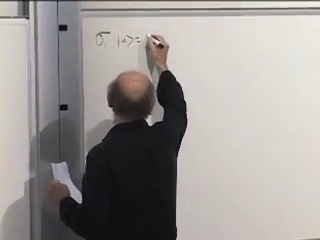
\includegraphics[width=0.62\linewidth]{lecture_05_figure_02.png}
\caption{جدول تأثيرات باولي الكامل المستخدم طوال المقارنة.}
\lectureframe{00:03:15}
\end{figure}

ليس لأي من لفّي المكونين اتجاه مفضل في أي من الحالتين:
\begin{equation}
  \expect{\sigma_i}_{\psi_\pm}=0,
  \qquad
  \expect{\tau_i}_{\psi_\pm}=0,
  \qquad i=1,2,3.
  \label{eq:l05-local-zero}
\end{equation}
فعلى سبيل المثال، يعطي الفحص الصريح المطلوب للحالة الموجبة
\begin{align}
  \bra{\psi_+}\sigma_3\ket{\psi_+}
  &=
  \frac12
  \bigl(\bra{ud}+\bra{du}\bigr)
  \bigl(\ket{ud}-\ket{du}\bigr)\nonumber\\
  &=
  \frac12(1-1)=0.
  \label{eq:l05-sigma3-expectation}
\end{align}
وتتلاشى الحدود المتصالبة لأن \(\braket{ud}{du}=0\).

\begin{figure}[htbp]
\centering
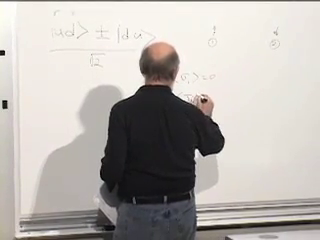
\includegraphics[width=0.78\linewidth]{lecture_05_figure_03.png}
\caption{تُحسب القيمة المتوقعة للحالة الموجبة بالتأثير بـ \(\sigma_3\) وباستخدام التعامد.}
\lectureframe{00:07:00}
\end{figure}

\begin{classroomqa}
\lecturetimestamp{00:07:13}
\audiencequestion{هل تعني القيمة المتوقعة الصفرية أنه يمكن قياس لف مفرد بحيث تكون قيمته صفرًا؟}
\lecturerresponse{لا. فمركبة من لف واحد لا تملك إلا النتيجتين \(+1\) و\(-1\)؛ وليس لـ \(\sigma_i\) أي قيمة ذاتية صفرية. تقول المعادلة~\eqref{eq:l05-local-zero} إن القياسات المتكررة تشبه رمية عملة عادلة، لا إن أي نتيجة فردية تساوي الصفر.}
\end{classroomqa}

إذن فقد فشل أول اختبار تشخيصي معقول. لا تستطيع المتوسطات المحلية أن تكشف الإشارة النسبية، لذا يجب أن نقيس خاصية للزوج.

\section{اللف الكلي يحدد الحالة الأحادية}

يُمثَّل العزم المغناطيسي للزوج بالمجموع المتجهي
\begin{equation}
  \boldsymbol{\Sigma}
  =
  \boldsymbol{\sigma}+\boldsymbol{\tau}.
\end{equation}
وتفني مركبته الثالثة متجهي الأساس كليهما:
\begin{align}
  (\sigma_3+\tau_3)\ket{ud}
  &=(1-1)\ket{ud}=0,\nonumber\\
  (\sigma_3+\tau_3)\ket{du}
  &=(-1+1)\ket{du}=0.
\end{align}
وبالتالي،
\begin{equation}
  (\sigma_3+\tau_3)\ket{\psi_\pm}=0.
\end{equation}
وكلا اختياري الإشارة له مركبة ثالثة كلية صفرية في كل تجربة.

أما المركبة الأولى فتميز بينهما. فمن المعادلة~\eqref{eq:l05-pauli-actions}،
\begin{align}
  (\sigma_1+\tau_1)\ket{ud}
  &=\ket{dd}+\ket{uu},\nonumber\\
  (\sigma_1+\tau_1)\ket{du}
  &=\ket{uu}+\ket{dd}.
\end{align}
ومن ثم
\begin{align}
  (\sigma_1+\tau_1)\ket{\psi_+}
  &=
  \sqrt2\bigl(\ket{uu}+\ket{dd}\bigr),\nonumber\\
  (\sigma_1+\tau_1)\ket{\psi_-}
  &=0.
  \label{eq:l05-total-x}
\end{align}
قد تكون القيمة المتوقعة لهذا المرصود في الحالة الموجبة صفرًا، لكنها ليست حالته الذاتية ذات القيمة الذاتية الصفرية.

\begin{classroomqa}
\lecturetimestamp{00:13:02}
\audiencequestion{ما النتائج التي يمكن أن تتخذها المركبة الكلية عندما لا تُفنى الحالة؟}
\lecturerresponse{إن إجابة كل مكوِّن هي \(+1\) أو \(-1\)، ولذلك يمكن أن يكون مجموعهما \(2\) أو \(0\) أو \(-2\). ولا تفرض القيمة المتوقعة الصفرية أن تكون النتيجة صفرًا في كل تجربة.}
\end{classroomqa}

وتكمل المركبة الثانية الاختبار. فمعاملاتها من \(i\) تتلاشى في التركيب المضاد للتناظر:
\begin{equation}
  (\sigma_2+\tau_2)\ket{\psi_-}=0.
\end{equation}
ولذلك تُفني المركبات الثلاث كلها الحالة السالبة،
\begin{equation}
  \bigl(\boldsymbol{\sigma}+\boldsymbol{\tau}\bigr)
  \cdot\hat n\,\ket{\psi_-}=0
  \qquad\text{for every unit vector }\hat n.
  \label{eq:l05-singlet-any-axis}
\end{equation}

\begin{figure}[htbp]
\centering
\includegraphics[width=0.84\linewidth]{lecture_05_figure_06.png}
\caption{الإلغاءات على مستوى كل مركبة التي تحدد الحالة السالبة بوصفها ذات لف كلي صفري.}
\lectureframe{00:16:30}
\end{figure}

الحالة المضادة للتناظر \(\ket{\psi_-}\) هي \emph{الأحادية}. وهي غير متغيرة دورانيًا: فكل محور يعطي الجواب نفسه للّف الكلي، وهو الصفر. أما الحالة المتناظرة في المعادلة~\eqref{eq:l05-two-signs} فتنتمي إلى القطاع الثلاثي.

\begin{classroomqa}
\lecturetimestamp{00:19:06}
\audiencequestion{هل تكون نتيجة اللفين المتعاكسين صحيحة في المتوسط فقط؟}
\lecturerresponse{بالنسبة إلى الأحادية، هي صحيحة في كل تجربة. فالمعادلة~\eqref{eq:l05-singlet-any-axis} هي معادلة متجه ذاتي، لذا فإن قياس المركبة نفسها على الجسيمين يعطي دائمًا إجابتين مجموعهما القيمة الذاتية الصفرية.}
\end{classroomqa}

\begin{classroomqa}
\lecturetimestamp{00:19:36}
\audiencequestion{لماذا تسمى الحالة الأخرى ثلاثية؟}
\lecturerresponse{تأتي هذه التسمية من الحالات الثلاث في المضاعف ذي اللف الكلي الواحد. ويؤجل اشتقاق ذلك؛ فالحساب الحالي لا يحتاج إلا إلى التباين بين الحالة المتناظرة وقطاع الأحادية ذي البعد الواحد.}
\end{classroomqa}

إذا قاس بوب أي مركبة من إلكترونه، عرف على الفور ما الذي كانت ستحصل عليه أليس لو قاست المركبة نفسها من إلكترونها: لا بد أن تكون إجابتها معاكسة. هذا ترابط أينشتاين--بودولسكي--روزن. ويمكن لزوج من العملات المخفية أيضًا أن يحمل نتيجتين متعاكستين، ولكن لسؤال واحد متفق عليه سلفًا فقط. أما الحالة الأحادية فتوفّر ترابطًا مضادًا تامًا لأي محور مكاني يُختار.

\begin{classroomqa}
\lecturetimestamp{00:20:55}
\audiencequestion{أكان أينشتاين وبودولسكي وروزن أولَ من اكتشف التشابك؟}
\lecturerresponse{لا. ناقش شرودنغر هذه الظاهرة وأدخل لغة التشابك. وجعلت حجة EPR مشكلة الارتباطات البعيدة حادّة على نحو خاص.}
\end{classroomqa}

\begin{classroomqa}
\lecturetimestamp{00:23:50}
\audiencequestion{هل ينتهك الترابط الفوري السببية، وهل يهم أي الراصدين يقيس أولًا؟}
\lecturerresponse{لا تُنقل أي رسالة قابلة للاستخدام. تبقى نتائج أليس المحلية متساوية الاحتمال، سواء قاس بوب أم لم يقس، في أي ترتيب قصوري. ولا تستطيع التحقق من الترابط إلا بعد أن تتلقى نتيجة بوب عبر قناة كلاسيكية عادية لا يمكنها أن تتجاوز الضوء.}
\end{classroomqa}

\section{متباينة بيل هي عد كلاسيكي}

قد يبدو وضع نتيجة بيل غير مستقر. ففي بعض الأيام تبدو أعمق سمة في ميكانيكا الكم؛ وفي أيام أخرى تبدو مجرد نتيجة حتمية أخرى للصياغة الشكلية. وكان بوسع بيل نفسه، وكذلك فاينمان، أن يعبرا عن الموقفين كليهما. غير أن المتباينة نفسها أولية. والمفاجأة تكمن في انتهاكها.

خذ مجموعة عادية من العناصر. يمكن لكل عنصر أن يملك أو ألا يملك ثلاث خواص \(A\) و\(B\) و\(C\). وليدل \(N(A,\neg B)\) على عدد العناصر التي لها \(A\) وليس لها \(B\). ويستلزم منطق المجموعات الكلاسيكي
\begin{equation}
  N(A,\neg B)+N(B,\neg C)
  \geq
  N(A,\neg C).
  \label{eq:l05-bell-count}
\end{equation}
والبرهان هو الاحتواء المجموعي
\begin{equation}
  A\cap C^{c}
  \subseteq
  (A\cap B^{c})\cup(B\cap C^{c}).
  \label{eq:l05-set-inclusion}
\end{equation}
ففي الواقع، ينتمي عنصر من \(A\cap C^c\) إما إلى \(B\) أو لا ينتمي إليه. وفي الحالة الأولى ينتمي إلى \(B\cap C^c\)؛ وفي الثانية ينتمي إلى \(A\cap B^c\). ولا يمكن لعد الاتحاد إلا أن يبالغ في عد المجموعة التي على اليسار.

\begin{figure}[htbp]
\centering
\includegraphics[width=0.78\linewidth]{lecture_05_figure_07.png}
\caption{يقسم البرهان على اللوح ثلاثة أجزاء فرعية كلاسيكية متداخلة إلى مناطق ذات أعداد غير سالبة.}
\lectureframe{00:31:15}
\end{figure}

وبصورة مكافئة، سمِّ المناطق المنفصلة في مخطط المجموعات الثلاث بالأعداد الصحيحة غير السالبة \(N_i\). ويحتوي طرفا المعادلة~\eqref{eq:l05-bell-count} على المناطق التي يقتضيها \(A\cap C^c\)، بينما يحتوي الطرف الأيسر على مناطق إضافية غير سالبة. ولم يدخل أي شيء كمومي بعد. فهذه مبرهنة عن المجموعات الجزئية والبدائل المنطقية العادية.

\section{تحويل عبارة المجموعات إلى تجربة لف مغزلي}

حضّر عددًا كبيرًا من أزواج الإلكترونات المستقلة في الحالة الأحادية، وعرّف ثلاث قضايا عن الإلكترون 1:
\begin{align}
  A&:\ \text{spin 1 is up at }0^\circ\text{, along the third axis},\nonumber\\
  B&:\ \text{spin 1 is up at }45^\circ\text{ in the }zx\text{-plane},\nonumber\\
  C&:\ \text{spin 1 is up at }90^\circ\text{, along the first axis}.
  \label{eq:l05-abc}
\end{align}

\begin{figure}[htbp]
\centering
\includegraphics[width=0.82\linewidth]{lecture_05_figure_08.png}
\caption{تُثبَّت قضايا اللف الثلاث عند \(0^\circ\) و\(45^\circ\) و\(90^\circ\) في مستوى واحد.}
\lectureframe{00:39:00}
\end{figure}

في الحالة الأحادية، يمكن إعادة صياغة نفي قضية عن الإلكترون 1 على أنه قضية موجبة عن الإلكترون 2. فعلى سبيل المثال،
\begin{align}
  \neg B
  &:\ \text{spin 1 is down at }45^\circ\nonumber\\
  &\Longleftrightarrow
  \text{spin 2 is up at }45^\circ.
\end{align}
وبالمثل، تصبح \(\neg C\) العبارة القائلة إن الإلكترون 2 إلى أعلى عند \(90^\circ\).

\begin{classroomqa}
\lecturetimestamp{00:40:04}
\audiencequestion{ألا ينبغي أن يجعل \(\neg C\) الإلكترون 2 إلى أسفل عند \(90^\circ\)؟}
\lecturerresponse{لا. أولًا انْفِ \(C\): يكون الإلكترون 1 إلى أسفل عند \(90^\circ\). ثم يجعل الترابط المضاد التام في الحالة الأحادية الإلكترون 2 إلى أعلى على ذلك المحور نفسه. ويجب إبقاء العكسين منفصلين.}
\end{classroomqa}

في عينة كبيرة، لا تختلف الأعداد والاحتمالات إلا بعامل هو العدد المشترك للأزواج المحضّرة. ويعطي عدم التغير الدوراني أيضًا
\begin{equation}
  P(A,\neg B)=P(B,\neg C),
\end{equation}
لأن التجربة الثانية هي الأولى نفسها بعد تدويرها بمقدار \(45^\circ\). ولذلك ستقتضي متباينة بيل الكلاسيكية
\begin{equation}
  2P(A,\neg B)\geq P(A,\neg C).
  \label{eq:l05-bell-probability}
\end{equation}
ونحتاج الآن إلى طريقة فعالة لحساب هذه الاحتمالات.

\section{تصبح القضايا مؤثرات إسقاط}

في فضاء متجهي عادي ثلاثي الأبعاد، يحذف المُسقِط كل مركبة متعامدة على فضاء جزئي مختار. فالمُسقِط أحادي البعد يُسقِط متجهًا إسقاطًا متعامدًا على مستقيم؛ والمُسقِط ثنائي البعد يُسقطه على مستوى. وإذا كان \(P\) يُسقِط على فضاء جزئي محدد، فـ
\begin{equation}
  P\ket{\alpha}=\ket{\alpha_P}.
\end{equation}

\begin{figure}[htbp]
\centering
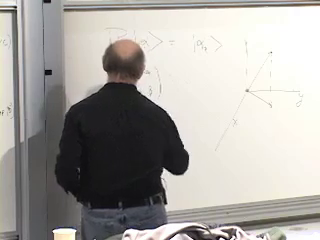
\includegraphics[width=0.76\linewidth]{lecture_05_figure_04.png}
\caption{يُعرض الإسقاط الهندسي وترميزه المؤثري جنبًا إلى جنب.}
\lectureframe{00:49:53}
\end{figure}

\begin{figure}[htbp]
\centering
\begin{tikzpicture}[scale=1.05,>=Latex]
  \draw[->] (-0.25,0)--(4.0,0);
  \draw[thick] (-0.25,-0.25)--(3.55,2.6);
  \draw[->,very thick] (0,0)--(2.25,3.05)
    node[above] {\(\ket{\alpha}\)};
  \coordinate (P) at (2.72,1.98);
  \draw[dashed] (2.25,3.05)--(P);
  \draw[->,very thick] (0,0)--(P)
    node[right] {\(\ket{\alpha_P}\)};
  \node[below right] at (3.1,2.25) {projected subspace};
\end{tikzpicture}
\caption{إعادة بناء واضحة لهندسة الإسقاط.}
\end{figure}

في فضاء هيلبرت لسبين واحد، تقابل القضية القائلة بأن \(\sigma_3=+1\) الفضاءَ الجزئي أحادي البعد المولَّد بواسطة \(\ket{u}\). ويعمل مسقِّطه على النحو الآتي
\begin{equation}
  P_{\sigma_3=+1}
  \begin{pmatrix}\alpha\\\beta\end{pmatrix}
  =
  \begin{pmatrix}\alpha\\0\end{pmatrix},
  \qquad
  P_{\sigma_3=-1}
  \begin{pmatrix}\alpha\\\beta\end{pmatrix}
  =
  \begin{pmatrix}0\\\beta\end{pmatrix}.
  \label{eq:l05-projector-actions}
\end{equation}

\begin{classroomqa}
\lecturetimestamp{00:49:55}
\audiencequestion{هل يبيّن المسقِّط الأول إلى أي ارتفاع يصل المتجه على محور رأسي؟}
\lecturerresponse{لا. إنه يكتفي بحذف المعامل المتعامد \(\beta\). فالمركبات سعات في فضاء هيلبرت، وليست إحداثيات مكانية اعتيادية للسبين.}
\end{classroomqa}

\begin{figure}[htbp]
\centering
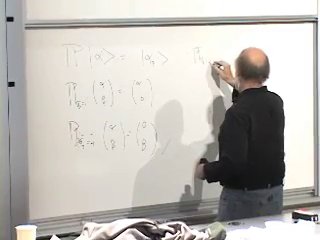
\includegraphics[width=0.78\linewidth]{lecture_05_figure_05.png}
\caption{تؤثِّر المسقِّطات أولًا في سبينور عام، ثم تُكتب بعد ذلك على صورة مصفوفات صريحة.}
\lectureframe{00:51:40}
\end{figure}

وصيغته المصفوفية هي
\begin{equation}
  P_{\sigma_3=+1}
  =
  \begin{pmatrix}1&0\\0&0\end{pmatrix}
  =
  \frac{I+\sigma_3}{2}.
  \label{eq:l05-p3}
\end{equation}
ويصلح البناء نفسه لأي متجه وحدة \(\hat n\):
\begin{equation}
  P_{\boldsymbol{\sigma}\cdot\hat n=+1}
  =
  \frac{I+\boldsymbol{\sigma}\cdot\hat n}{2}.
  \label{eq:l05-pn}
\end{equation}

\begin{classroomqa}
\lecturetimestamp{00:53:09}
\audiencequestion{ما المسقِّط على \(\sigma_1=+1\)؟}
\lecturerresponse{استبدل \(\sigma_3\) بـ \(\sigma_1\) في المعادلة~\eqref{eq:l05-p3}: \(P_{\sigma_1=+1}=(I+\sigma_1)/2\).}
\end{classroomqa}

تأخذ قاعدة بورن الآن صيغة مفيدة للقضايا:
\begin{equation}
  P(\mathcal A\text{ is true in }\ket{\psi})
  =
  \bra{\psi}P_{\mathcal A}\ket{\psi}.
  \label{eq:l05-projector-born}
\end{equation}
وبالنسبة إلى سبينور مطبَّع \(\ket{\psi}=(\alpha,\beta)^T\)، فإن المعادلة~\eqref{eq:l05-projector-born} مع \(P_{\sigma_3=+1}\) تعطي \(|\alpha|^2\)، كما ينبغي تمامًا.

تكشف هذه اللغة الفرق بين القضايا الكلاسيكية والقضايا الكمية. ففي المنطق الكلاسيكي، تقابل الخاصية مجموعةً جزئية من مجموعة. وفي ميكانيكا الكم، تقابل الخاصية فضاءً جزئيًا من فضاء هيلبرت، أو على نحو مكافئ مسقِّطها. ولا تخضع المجموعات الجزئية والفضاءات الجزئية المتجهية لعمليات الشبكة نفسها؛ ومن ذلك الاختلاف ينشأ تناقض بيل.

\subsection{المسقِّط المشترك لبيل}

بالنسبة إلى \(A\wedge\neg B\)، يجب أن يكون إلكترون 1 في حالة سبين لأعلى على طول المحور الثالث، ويجب أن يكون إلكترون 2 في حالة سبين لأعلى على طول
\begin{equation}
  \hat n_{45}=\frac{\hat x+\hat z}{\sqrt2}.
\end{equation}
ومركبة السبين المعنية للجسيم الثاني هي
\begin{equation}
  \boldsymbol{\tau}\cdot\hat n_{45}
  =
  \frac{\tau_1+\tau_3}{\sqrt2}.
\end{equation}
ولذلك يكون المسقِّط المشترك
\begin{equation}
  P_{A\wedge\neg B}
  =
  \frac{I+\sigma_3}{2}
  \frac{I+(\tau_1+\tau_3)/\sqrt2}{2}.
  \label{eq:l05-joint-projector}
\end{equation}

\begin{classroomqa}
\lecturetimestamp{00:59:18}
\audiencequestion{لماذا يوجد عامل \(1/\sqrt2\) في مركبة السبين ذات \(45^\circ\)؟}
\lecturerresponse{يجب أن يكون الاتجاه متجهَ وحدة. فمركبتاه على المحورين الأول والثالث كلتاهما \(1/\sqrt2\)، لذا فإن المرصود الموافق هو \((\tau_1+\tau_3)/\sqrt2\).}
\end{classroomqa}

\begin{classroomqa}
\lecturetimestamp{01:00:52}
\audiencequestion{هل التعبير كله \(I+\boldsymbol{\tau}\cdot\hat n_{45}\) مقسوم على اثنين؟}
\lecturerresponse{نعم. فالمسقِّط هو \(\bigl(I+\boldsymbol{\tau}\cdot\hat n_{45}\bigr)/2\)؛ والعامل \(1/2\) يضرب البسط كله.}
\end{classroomqa}

العاملان في المعادلة~\eqref{eq:l05-joint-projector} يؤثران في عاملين مختلفين من الجداء التنسوري ويتبادلان. وتطبيقهما معًا يزيل أولًا كل مركبة يكون فيها إلكترون 1 في حالة سبين لأسفل، ثم كل مركبة باقية يكون فيها إلكترون 2 في حالة سبين لأسفل على طول \(\hat n_{45}\).

\section{الأعداد الكمية تقلب المتباينة}

لنرمز بـ
\begin{equation}
  \ket{\psi_s}
  =
  \frac{\ket{ud}-\ket{du}}{\sqrt2}
\end{equation}
إلى الحالة الأحادية. نبدأ من
\begin{equation}
  P(A,\neg B)
  =
  \bra{\psi_s}P_{A\wedge\neg B}\ket{\psi_s}.
\end{equation}
العامل \((I+\sigma_3)/2\) يلغي \(\ket{du}\) ويُبقي \(\ket{ud}/\sqrt2\). ثم يعطي العامل الثاني
\begin{align}
  \frac{I+(\tau_1+\tau_3)/\sqrt2}{2}\ket{ud}
  &\notag\\[-0.3em]
  &=
  \frac12
  \left[
    \ket{ud}
    +\frac{\ket{uu}-\ket{ud}}{\sqrt2}
  \right]\nonumber\\
  &=
  \frac12
  \Biggl[
    \left(1-\frac1{\sqrt2}\right)\ket{ud}
  \nonumber\\
  &\qquad
    +\frac1{\sqrt2}\ket{uu}\Biggr].
  \label{eq:l05-projector-action}
\end{align}
وللحد \(\ket{uu}\) تراكب صفري مع برا الحالة الأحادية، وتعطي عوامل التطبيع الباقية
\begin{equation}
  P(A,\neg B)
  =
  \frac14\left(1-\frac1{\sqrt2}\right).
  \label{eq:l05-pab}
\end{equation}

\begin{figure}[htbp]
\centering
\includegraphics[width=0.88\linewidth]{lecture_05_figure_09.png}
\caption{يبقي حساب المسقِّط على تراكب \(\ket{ud}\) ويستبعد المساهمة المتعامدة \(\ket{uu}\).}
\lectureframe{01:08:20}
\end{figure}

يعطي التناظر الدوراني النتيجة نفسها للزوج التالي من الاتجاهات:
\begin{equation}
  P(B,\neg C)
  =
  \frac14\left(1-\frac1{\sqrt2}\right).
\end{equation}
وبالنسبة إلى \(A\wedge\neg C\)، يكون المحور الثاني هو المحور المكاني الأول، ولذا
\begin{equation}
  P_{A\wedge\neg C}
  =
  \frac{I+\sigma_3}{2}\frac{I+\tau_1}{2}.
\end{equation}
ويُبقي العامل الأول مرة أخرى \(\ket{ud}/\sqrt2\). ويولِّد الحد \(\tau_1\) الحالة \(\ket{uu}\)، وهي متعامدة مع برا الحالة الأحادية، بينما يبقى حد الهوية. ومن ثم
\begin{equation}
  P(A,\neg C)=\frac14.
  \label{eq:l05-pac}
\end{equation}
وبجمع النتائج الثلاث،
\begin{equation}
  \underbrace{
  P(A,\neg B)+P(B,\neg C)
  }_{\frac12(1-1/\sqrt2)\approx0.146}
  <
  \underbrace{
  P(A,\neg C)
  }_{\frac14=0.25}.
  \label{eq:l05-bell-violation}
\end{equation}

\begin{figure}[htbp]
\centering
\includegraphics[width=0.84\linewidth]{lecture_05_figure_10.png}
\caption{يعرض الحساب المكتمل على اللوح الطرف الأيسر الأصغر في متباينة بيل والطرف الأيمن الأكبر.}
\lectureframe{01:12:15}
\end{figure}

تقلب المعادلة~\eqref{eq:l05-bell-violation} المعادلة~\eqref{eq:l05-bell-probability}. وليس الاستنتاج أن ميكانيكا الكم تناقض نفسها. بل إن المقصود هو أن ارتباطات الحالة الأحادية لا يمكن أن تنشأ من نموذج كلاسيكي محلي تكون فيه قضايا السبين الثلاث كلها ذات قيم صدق اعتيادية من نوع نظرية المجموعات، مستقلة عن اختيار القياس البعيد. ولا تستطيع محاكاة كلاسيكية إعادة إنتاج تلك الارتباطات إلا بالتخلي عن فرض واحد على الأقل من فروض بيل، وأبرزها المحلية.

\section{ما الذي تختبره تجربة بيل}

تتنبأ ميكانيكا الكم بالفعل بانتهاك المتباينة. ويجب على التجربة، بالإضافة إلى ذلك، أن تسد طريق الإفلات الكلاسيكي الذي يُعلِم فيه أحد الكاشفين الآخر بالإعداد أو بالنتيجة التي صادفها. وينبغي أن يكون جناحا التجربة متباعدين بما يكفي، وأن تكون الاختيارات وعمليات الكشف متقاربة بما يكفي زمنيًا، بحيث لا تتمكن إشارة بسرعة الضوء من الانتقال بينهما. وجعلت تجربة Aspect ذلك التوقيت وذلك العزل مقنعين من الناحية التشغيلية.

\begin{classroomqa}
\lecturetimestamp{01:13:15}
\audiencequestion{إذا كانت ميكانيكا الكم تعطي الجواب بالفعل، فهل علَّمتنا تجارب بيل شيئًا؟}
\lecturerresponse{لقد اختبرت ما إذا كانت الطبيعة تتبع التنبؤ الكمي في تجربة الارتباط هذه تحديدًا، وجعلت، على نحو حاسم، جناحي القياس مستقلين على مقياس زمن انتقال الضوء ذي الصلة. وكان الضبط التجريبي والتوقيت في حد ذاتهما إنجازين كبيرين.}
\end{classroomqa}

\begin{classroomqa}
\lecturetimestamp{01:18:19}
\audiencequestion{ماذا أضاف بيل بعد مناقشة أينشتاين للتأثير الشبحي عن بُعد؟}
\lecturerresponse{قدَّم بيل متباينة كمية. وحدد تجربة ارتباط قابلة للتنفيذ يستبعد تنبؤها الكمي تفسيرًا أساسيًا كلاسيكيًا محليًا، بدلًا من ترك الاعتراض عند مستوى الانزعاج الفلسفي. وظل موقف بيل ملتبسًا إزاء ما إذا كان ذلك حتميًا أم عميق الدلالة، وأصبح تدريجيًا أكثر استعدادًا للتشكيك في ميكانيكا الكم القياسية.}
\end{classroomqa}

قد تفصل بين الجسيمين أميال مع بقائهما متشاركين في حالة مشتركة واحدة، لكن هذا يظل تجربة كمية على أنظمة صغيرة. وتميل تفاعلات البيئة إلى تدمير العلاقات الطورية المطلوبة. ويمكن لجزيئات الهواء والفوتونات الشاردة والاضطرابات الحرارية أن تتشابك مع الزوج، لذا يجب أن يُجرى الفصل بينهما في بيئة باردة جيدة العزل.

\begin{classroomqa}
\lecturetimestamp{01:19:53}
\audiencequestion{هل تجعل حالة مشتركة ممتدة عبر مسافة كبيرة من هذا جسمًا كميًا عيانيًا؟}
\lecturerresponse{الأفضل وصفه على أنه أنظمة كمية صغيرة متباعدة. قد تكون المسافة الفاصلة بينها كبيرة، لكن الحفاظ على دالتها الموجية المشتركة يغدو أكثر حساسية لأن التفاعل غير المضبوط مع البيئة يدمّر التماسك المفيد. كرتا بولينغ عاديتان لا تتيحان التجربة نفسها.}
\end{classroomqa}

\begin{classroomqa}
\lecturetimestamp{01:21:23}
\audiencequestion{هل يمكن لقياس أحد الجسيمين أن يكشف معلومات متممة عن الآخر، وبذلك يتجاوز مبدأ عدم اليقين؟}
\lecturerresponse{يمكن، على سبيل المثال، قياس موضع أحد الجسيمين وزخم الآخر. وهذا ليس قياسًا متزامنًا لمرصودين لا يتبادلان على جسيم واحد. ولم يُتجاوز قيد عدم اليقين على نظام مفرد.}
\end{classroomqa}

\section{متى يدل حاصل الضرب على «و»؟}

تضمَّن حساب بيل ضرب مسقِّطين. وهذا لا يمثّل اقترانًا إلا للقضايا المتوافقة.

\begin{classroomqa}
\lecturetimestamp{01:22:39}
\audiencequestion{لماذا مثّل حاصل ضرب مسقِّطين الكلمة المنطقية «و»؟}
\lecturerresponse{لأن المسقِّطين يتبادلان. يؤثر أحدهما في إلكترون 1 والآخر في إلكترون 2، لذا لا يهم ترتيبهما ويمكن اختبار الخاصيتين معًا. أما لإلكترون واحد، فإن \((I+\sigma_3)/2\) و\((I+\sigma_1)/2\) لا يتبادلان؛ فحالة السبين لأعلى على طول كلا المحورين ليست قضية محددة معًا من هذا النوع.}
\end{classroomqa}

هذا موضع آخر تفارق فيه القضايا الكمية المجموعات الجزئية العادية. فالتقاطع الكلاسيكي موجود دائمًا. أما النظير الكمي الذي يمثله مسقِّط حاصل الضرب فلا يملك المعنى المنطقي المقصود إلا حين تكون الفضاءات الجزئية المعنية متوافقة.

ويشير هذا النقاش نفسه إلى القياس ذاته. فلجهاز القياس حالة مؤشر. فإذا دفع إلكترون في حالة سبين لأعلى المؤشر في اتجاه، ودفع إلكترون في حالة سبين لأسفل المؤشر في اتجاه آخر، فإن إلكترونًا في حالة تراكب يصبح متشابكًا مع موضعين للمؤشر. ولذا يمكن دراسة القياس بوصفه تشابكًا بين النظام والجهاز. غير أن هذه المسألة تُؤجَّل لصالح مبرهنة أقصر لا تستخدم إلا الخطية.

\begin{classroomqa}
\lecturetimestamp{01:25:09}
\audiencequestion{هل من المفيد النظر إلى انهيار الدالة الموجية على أنه قياس واحد يقيِّد الحالة المشتركة؟}
\lecturerresponse{ينتمي هذا السؤال إلى عملية القياس. إذ يتشابك الجهاز والنظام المقاس: ترتبط إحدى قيم السبين بموضع للمؤشر، وترتبط القيمة الأخرى بموضع آخر. وقد أُرجئ النقاش التفصيلي للقياس.}
\end{classroomqa}

\section{الخطية تمنع آلة نسخ كونية}

لا نحتاج إلا إلى حقيقة واحدة عن التطور الزمني. فإذا حوَّلت عملية فيزيائية
\begin{equation}
  \ket{a}\longrightarrow\ket{a'},
  \qquad
  \ket{b}\longrightarrow\ket{b'},
\end{equation}
فإن الخطية تقتضي
\begin{equation}
  \alpha\ket{a}+\beta\ket{b}
  \longrightarrow
  \alpha\ket{a'}+\beta\ket{b'}.
  \label{eq:l05-linearity}
\end{equation}

يمكن لآلة نسخ عادية أن تعيد إنتاج المعلومات الكلاسيكية بأخطاء صغيرة يمكن التحكّم فيها. أما المطلب الكمي فأقوى: إذ يجب على جهاز واحد بعينه أن ينسخ سعات أي حالة تُعرَض عليه كاملةً. ولهذا يُسمّى مبدأ عدم الاستنساخ أيضًا مبدأ عدم وجود آلة Xerox كمومية.

تخيّل آلة لها منفذ إدخال واحد ومنفذا إخراج. إذا كانت تستنسخ أساس المحور الثالث، فلا بد أن تنفّذ
\begin{equation}
  \ket{u}\longrightarrow\ket{uu},
  \qquad
  \ket{d}\longrightarrow\ket{dd}.
  \label{eq:l05-clone-basis}
\end{equation}
يمكن للآلة أن تزوّد مخرجيها بطاقة أو كتلة أو شحنة؛ فمسك حسابات الانحفاظ ليس هو العائق. بل إن التناقض يتعلق باعتماد التحويل على الحالة.

\begin{figure}[H]
\centering
\includegraphics[width=0.86\linewidth]{lecture_05_figure_11.png}
\caption{يُفترَض في جهاز افتراضي ذي مدخل واحد ومخرجين أن يستنسخ حالتي الأساس كلتيهما.}
\lectureframe{01:33:45}
\end{figure}

أدخِل الآن لفًّا مغزليًا يشير إلى اليمين،
\begin{equation}
  \ket{r}
  =
  \frac{\ket{u}+\ket{d}}{\sqrt2}.
  \label{eq:l05-right-state}
\end{equation}
فتفرض المعادلتان~\eqref{eq:l05-linearity} و\eqref{eq:l05-clone-basis} أن يكون الخرج
\begin{equation}
  \ket{r}
  \longrightarrow
  \frac{\ket{uu}+\ket{dd}}{\sqrt2}.
  \label{eq:l05-linear-output}
\end{equation}
أما الاستنساخ التام فيتطلب بدلًا من ذلك نسختين مستقلتين:
\begin{align}
  \ket{rr}
  &=
  \ket{r}\otimes\ket{r}\nonumber\\
  &=
  \frac12
  \left(
    \ket{uu}+\ket{ud}+\ket{du}+\ket{dd}
  \right).
  \label{eq:l05-cloned-output}
\end{align}
والحدود المختلطة في المعادلة~\eqref{eq:l05-cloned-output} غير موجودة في المعادلة~\eqref{eq:l05-linear-output}. لذا فالحالتان الناتجتان مختلفتان.

\begin{figure}[H]
\centering
\includegraphics[width=0.72\linewidth]{lecture_05_figure_12.png}
\caption{لا تنتج الخطية إلا حدود اللفّين المغزليين المتوازيين، في حين أن نسختين حقيقيتين مشيرتين إلى اليمين تحتويان أيضًا على كلا الحدّين المختلطين.}
\lectureframe{01:35:20}
\end{figure}

\begin{theorem}[No-cloning]
لا تستطيع أي آلة فيزيائية واحدة أن تستنسخ بدقة كل حالة كمومية مجهولة.
\end{theorem}

\begin{proof}
افترض أن آلة واحدة تستنسخ حالتي الأساس المتعامدتين كما في المعادلة~\eqref{eq:l05-clone-basis}. ثم تحدد الخطية خرجها على تراكبهما ليكون ما في المعادلة~\eqref{eq:l05-linear-output}. أما الاستنساخ التام للمدخل نفسه فيتطلب ما في المعادلة~\eqref{eq:l05-cloned-output}. ولأن متجهي الحالة مختلفان، فلا يمكن أن توجد الآلة الشاملة المفترضة.
\end{proof}

والسبب بنيوي. فتحويل \(\ket{\psi}\) إلى \(\ket{\psi}\otimes\ket{\psi}\) تربيعي في السعات، في حين أن كل تطور مسموح به للحالة الكمومية الكاملة خطي.

\begin{classroomqa}
\lecturetimestamp{01:35:49}
\audiencequestion{هل يفترض البرهان أن المخرجين مستقلان؟}
\lecturerresponse{نعم، لأن المطلوب أن يمكن استعمال كل من النسختين على نحو مستقل. والأنظمة المستقلة تُركَّب بالجداء التنسوري، ولهذا تُمثَّل نسختان مشيرتان إلى اليمين بـ \(\ket{r}\otimes\ket{r}\). أما النواتج المترابطة التي لا يمكن استعمالها على حدة فليست نسختين.}
\end{classroomqa}

\begin{classroomqa}
\lecturetimestamp{01:37:20}
\audiencequestion{يبدو أن الليزر ينسخ حالة فوتون عن طريق الانبعاث المحفَّز. فأين يفشل هذا الاستدلال؟}
\lecturerresponse{تشارك الذرة وأنماط المجال الكهرومغناطيسي أيضًا. وتسهم حالة الذرة وتلك الأنماط في الخرج، وتظهر بوصفها ضجيجًا من منظور الاستنساخ الشامل. ويمكن تحقيق استنساخ تقريبي، لكن الاستنساخ التام غير المعتمد على الحالة غير ممكن.}
\end{classroomqa}

\begin{classroomqa}
\lecturetimestamp{01:40:24}
\audiencequestion{هل يمكن نقل المعلومات الكمومية رغم تعذّر استنساخها؟}
\lecturerresponse{نعم. فالنقل عملية مختلفة: لا يلزم أن يحتفظ الأصل بالحالة. إن عدم الاستنساخ يمنع الوصول في النهاية إلى نسختين مستقلتين متطابقتين تمامًا، لا نقل الحالة من حامل إلى آخر.}
\end{classroomqa}

\begin{classroomqa}
\lecturetimestamp{01:41:03}
\audiencequestion{هل يجب أن تكون حالة الإدخال مجهولة؟}
\lecturerresponse{إذا كانت الحالة معلومة سلفًا، فيمكن إعداد مزيد من الأنظمة في تلك الحالة، أو بناء جهاز مكيَّف مع أساس متعامد مختار. أما المستحيل فهو آلة واحدة تقبل مدخلًا اعتباطيًا وتستنسخه من غير معرفة مسبقة بالحالة التي وصلت.}
\end{classroomqa}

\begin{classroomqa}
\lecturetimestamp{01:42:35}
\audiencequestion{أي التعبيرين عن الحالة اليمنى هو الخرج الفعلي للآلة؟}
\lecturerresponse{تفرض الخطية المعادلة~\eqref{eq:l05-linear-output}؛ بينما يقتضي الاستنساخ المعادلة~\eqref{eq:l05-cloned-output}. وهذا الاختلاف بينهما هو التناقض بعينه.}
\end{classroomqa}

\begin{classroomqa}
\lecturetimestamp{01:43:40}
\audiencequestion{هل يمكن قياس المعلومات الإضافية التي تحملها حالات الجسيمين المتشابكة كمّيًا؟}
\lecturerresponse{لحالة نقية للَّفٍّ مغزلي واحد معامِلان فيزيائيان حقيقيان. ويوفّر لفّان مغزليان أُعِدّا كلٌّ على حدة أربعة معلمات، في حين أن حالة نقية عامة في فضاء هيلبرت رباعي الأبعاد للَّفَّين المغزليين لها ستة معلمات بعد حذف التطبيع والطور الكلي. وتشمل الحالات الإضافية حالات متشابكة، ويمكن قياس درجة تشابكها بإنتروبيا التشابك.}
\end{classroomqa}

\enlargethispage{4\baselineskip}
لقد أدّت الإشارة في المعادلة~\eqref{eq:l05-two-signs} الآن ثلاث وظائف. فقد اختارت الحالة الوحيدة ذات اللفّ الكلي الصفري، ووفّرت ترابطات تنتهك متباينة مجموعات كلاسيكية، وكشفت الفرق بين تطور كمومي خطي والفعل اللاخطي المتمثل في صنع نسختين. وينشأ كلٌّ من هذه النتائج من التعامل مع الحالة المشتركة بوصفها متجهًا في فضائها الكامل للجداء التنسوري، لا بوصفها قائمةً بخصائص موضعية موجودة سلفًا.
